\documentclass{beamer}
\usetheme{default}
\setbeamertemplate{navigation symbols}{}
%	
\usepackage{epstopdf}
\usepackage{subfig}
\usepackage{amsmath, amsthm, amssymb}
\usepackage{float}
\usepackage{rotating}
\usepackage{graphicx}
\usepackage{longtable}
\usepackage{xcolor}
\usepackage{bm}
\usepackage{tikz}
\usetikzlibrary{shapes}
\tikzset{My Arrow Style/.style={single arrow, fill=red!50, anchor=base, align=center,text width=.5cm,rotate =270}}
\newcommand{\MyArrow}[2][]{\tikz[baseline] \node [My Arrow Style,#1] {#2};}
\tikzset{My 2Arrow Style/.style={single arrow, fill=red!50, anchor=base, align=center,text width=.5cm,rotate =90}}
\newcommand{\MyArrowUp}[2][]{\tikz[baseline] \node [My 2Arrow Style,#1] {#2};}
\newcommand{\bmat}{\begin{matrix}}
\newcommand{\emat}{\end{matrix}}

\newtheorem{acknowledgement}[theorem]{Acknowledgement}
\newtheorem{algorithm}[theorem]{Algorithm}
\newtheorem{assumption}{Assumption}
\newtheorem{axiom}{Axiom}
\newtheorem{case}[theorem]{Case}
\newtheorem{claim}[theorem]{Claim}
\newtheorem{conclusion}[theorem]{Conclusion}
\newtheorem{condition}[theorem]{Condition}
\newtheorem{conjecture}{Conjecture}
\newtheorem{criterion}[theorem]{Criterion}
\newtheorem{proposition}{Proposition}
\newtheorem{summary}[theorem]{Summary}
\newtheorem{exercise}{Exercise}
\newtheorem{notation}{Notation}
\newtheorem{remark}{Remark}
%\graphicspath{{graphs//}}

\title {Taxes, Debts,  and Redistributions with Aggregate Shocks}
\author{Anmol Bhandari, David Evans, Mikhail Golosov, Thomas J. Sargent}

\date{September 2013}
% \today will show current date.
% Alternatively, you can specify a date.
%
\begin{document}
%
\begin{frame}
\titlepage

\end{frame}

\begin{frame}
\frametitle{Optimal Taxation Under Commitment With}

\begin{itemize}
 \item \textbf{Heterogeneous agents}

 \quad \color{red}$\rightarrow$ \color{black} Different productivities

 \item \textbf{Incomplete markets}

 \quad \color{red}$\rightarrow$ \color{black}All trade only a risk-free bond

 \item \textbf{Affine tax schedules}

 \quad \color{red}$\rightarrow$ \color{black}Government levies a proportional tax on labor earnings + lump sum (tax or transfer)

 \item \textbf{Aggregate shocks}

 \quad \color{red}$\rightarrow$ \color{black} To productivities, government expenditures, discount factors

 \end{itemize}
\end{frame}


\begin{frame}
\frametitle{Questions}

\begin{enumerate}
 \item How costly is government debt?
 \item What are the long run properties of optimal government policies and equilibrium allocations?
\item How should government policies respond to aggregate shocks?
\end{enumerate}

\end{frame}




\begin{frame}
 \frametitle{Environment}
 \begin{itemize}
 \item \textbf{Uncertainty}: Markov aggregate shocks $s_t$
  \item \textbf{Demography}: $I$ types of infinitely lived agents (of mass $\pi_i$)  plus a benevolent planner
  \item \textbf{Technology}: Output $\sum_{i=1}^I \theta_{i,t} l_{i,t}$ is linear in labor supplies. Productivities $\{\theta_i(s_t)\}_{i,t}$ differ across $i$.
  \item \textbf{Preferences }(Households)
  \begin{equation*}
\mathbb{E}_{0}\sum_{t=0}^{\infty } \bar{\beta}_t  U^{i}\left(
c_{i}(s^t),l_{i}(s^t)\right)  \label{utility lifetime}
\end{equation*}%
where 
$\bar{\beta}_t=\bigl[\Pi_{j=0}^{t-1} \beta(s_j) \bigr]$ %$\bar{\beta}_t=\beta(s_{t-1}) \bar{\beta}_{t-1}$ , $\beta(s)\in (0,1)$ and  $\beta(s_0)=1$
\item \textbf{Preferences} (Planner): Given Pareto weights $\{\alpha_i\}$
\begin{equation*}
\mathbb{E}_{0}\sum_{i=1}^{I}\pi _{i}\alpha _{i}\sum_{t=0}^{\infty }\bar{\beta}_t U_{t}^{i}\left( c_{i,t},l_{i,t}\right)  \label{govmt objective}
\end{equation*}
  \item \textbf{Asset Markets}: A risk-free bond only
  \end{itemize}

\end{frame}

\begin{frame}
 \frametitle{Environment, II}
 \begin{itemize}
  \item \textbf{Affine Taxes}: Agent $i$'s tax bill
\[- T_t + \tau_t \theta_{i,t}l_{i,t}\]

\item[]
  \item \textbf{Budget Constraints}
  \begin{itemize}
   \item Agent $i$: $ c_{i,t}+b_{i,t}=\left( 1-\tau _{t}\right) \theta _{i,t}l_{i,t}+R_{t-1}b_{i,t-1}+T_{t}$
\item Government: $g_{t}+B_{t}+T_t=\tau _{t}\sum_{i=1}^{I}\pi _{i}\theta_{i,t}l_{i,t}+R_{t-1}B_{t-1}$
  \end{itemize}

\item[]
  \item \textbf{Market Clearing}
  \begin{itemize}
   \item Goods: $\sum_{i=1}^{I}\pi_{i}c_{i,t}+g_t =\sum_{i=1}^{I}\pi
_{i}\theta _{i,t} l_{i,t}$

   \item Assets: $\sum_{i=1}^{I}\pi _{i}b_{i,t}+B_{t}=0$

  \end{itemize}
  \item[]

\item \textbf{Initial Distribution of Assets} $\{b_{i,-1}\}_i$ and $B_{-1}$
\end{itemize}
\end{frame}


\begin{frame}
 \frametitle{Ramsey Problem}

\begin{definition}
\textbf{Allocation, price system, government policy}: Standard

\end{definition}

\begin{definition}
\textbf{Competitive equilibrium}: Given $\left( \left\{ b_{i,-1}\right\}
_{i},B_{-1}\right) $ and $\left\{ \tau _{t},T_{t}\right\} _{t=0}^{\infty }$,
all allocations are chosen optimally, markets clear \footnote{Usually, we impose only  ``natural'' debt limits. }
\end{definition}

\begin{definition}
\textbf{Optimal competitive equilibrium}: A welfare-maximizing competitive
equilibrium for a given $\left( \left\{ b_{i,-1}\right\} _{i},B_{-1}\right) $
\end{definition}

 \end{frame}

\begin{frame}
\frametitle{Contrast with representative agent models}
 Representative agent and linear taxes
\begin{itemize}
 \item Higher levels of government debt are distortionary
 \item With incomplete markets (as in  AMSS), the optimal  government policy is to accumulate assets
 \end{itemize}

 \end{frame}
%
%  \begin{frame}
%  \frametitle{Does AMSS Confirm Reinhart-Rogoff Fears?}
%  \begin{itemize}
%  \item Higher govt.\ debts are more  distorting, but $\ldots$
%  \item Because it is distortionary, asymptotically govt. doesn't issue debt
%  \end{itemize}
%  Things change in our environment
%  \end{frame}

 \begin{frame}
 \frametitle{Redistribution and optimal transfers}
 \begin{itemize}
  \item Representative agent models restrict transfers
  \begin{itemize}
 \item Implicitly motivated by concerns about  redistribution:  poor people can't afford lump sum taxes
  \item These constraints almost always bind (e.g.,  Lucas Stokey, AMSS) and drive long-run govt debt dynamics
  \end{itemize}
\item We begin with explicit redistribution motive  and let the government set transfers optimally
 \end{itemize}

 \vspace{4mm}
 \color{red}\emph{Prescriptions for optimal tax-transfers differ substantially with explicitly modeled redistribution concerns}
 \end{frame}

\begin{frame}
 \frametitle{Main working parts}
\begin{itemize}
 \item \textbf{Welfare Criterion}: Benevolent planner with explicit redistribution motives
 \item \textbf{Instruments}: Transfers and a flat tax on labor income
 \item \textbf{Restrictions}:
 \begin{enumerate}
  \item The tax on labor income is linear in wage earnings
  \item Transfers are unrestricted in sign and magnitude  but cannot be  conditioned on agents' identities
  \item Incomplete markets
 \end{enumerate}
\item \textbf{Trade-offs}:
\begin{enumerate}
\item Changes in labor taxes impose dead weight losses
\item Explicit redistribution motives imply costs of fluctuating transfers. Withdrawing a unit of consumption affects rich and poor people differently
\end{enumerate}
\end{itemize}
\end{frame}
\begin{frame}
 \frametitle{Key forces }
 \begin{itemize}
  \item \textbf{Heterogeneity}
  \begin{enumerate}
  \item Two sources of heterogeneity: Productivities and asset holdings
   \item Unrestricted transfers $\rightarrow$ \emph{Level }of government debt is irrelevant; \emph{distribution} across agents matters

  E.G, high productivity agents owning more government debt can be more distortionary
  \end{enumerate}
  \item \textbf{Responses}

  Since welfare costs depend on the distribution of assets, optimal policy is affected by and affects the distribution of net assets
\begin{enumerate}
\item \textbf{Absence of agent-specific transfers}: This motivates  the govt. to engineer  a negative correlation between net assets and labor earnings
\item \textbf{Absence of state contingent securities}: This motivates the govt. to exploit endogenous fluctuations in the interest rate

 \end{enumerate}
\end{itemize}

\end{frame}

%
% \begin{frame}
% \frametitle{Key mechanisms}
% Two departures from representative agent models:
% \begin{itemize}
% \item \textbf{Unrestricted transfers}: Level of debt is not distortionary. What matters is how it is distributed across agents
%  \item \textbf{Explicit redistribution motives}: Endogenous costs of fluctuating transfers. Taking away a unit of consumption good affects ``rich'' and ``poor'' people differently
%  \end{itemize}
%
% \emph{One part of heterogeneity (productivities) is exogenous but heterogeneity in assets is endogenous. }
%
%
% \end{frame}



 \begin{frame}
  \frametitle{Ricardian Equivalence}
  \begin{itemize}
   \item \emph{Result}: A \textbf{large set} of transfers and asset profiles support the same competitive allocation
   \item \emph{Logic}: Withdrawing a unit of assets from all agents and increasing transfers by a unit leaves budget sets unchanged
  \end{itemize}
  \textbf{Notation}: $\tilde{b}_{i,t}=b_{i,t}-b_{1,t}$ be the \textbf{relative assets} of agent $i$
  \small
 \begin{theorem}
 Given $\left( \left \{ b_{i,-1}\right \} _{i},B_{-1}\right) $, let $\left \{ \left \{ \color{red}{c}_{i,t},l_{i,t},\color{black}b_{i,t}\right \} _{i},B_{t},\color{red}{R}_{t}\color{black}\right \} _{t} $ and $\left \{ \color{red}\tau _{t}\color{black},T_{t}\right\} _{t}$ be a competitive equilibrium.

 For any bounded sequences $\left \{ \hat{b}_{i,t}\right \} _{i,t\geq -1}$ that satisfy
 \begin{equation*}
 \hat{b}_{i,t}-\hat{b}_{1,t}=\tilde{b}_{i,t}\text{ for all }t\geq -1,i\geq 2,
 \end{equation*}%
 there exist  sequences $\left \{ \hat{T}_{t}\right \} _{t}$ and $%
 \left \{ \hat{B}_{t}\right \} _{t\geq -1}$ such that $\left \{ \left \{ \color{red}{c}_{i,t},l_{i,t}\color{black},\hat{b}%
 _{i,t}\right \} _{i},\hat{B}_{t},\color{red}{R}_{t}\color{black}\right \} _{t}$ and $\left \{
 \color{red}{\tau}_{t}\color{black},\hat{T}_{t}\right \} _{t}$ constitute a competitive
 equilibrium given $\left( \left \{ \hat{b}_{i,-1}\right \} _{i},\hat{B}%
 _{-1}\right) $.
 \end{theorem}
\end{frame}



%
% \begin{frame}
%  \frametitle{Ricardian Equivalence}
%  \begin{itemize}
%   \item \emph{Result}: A \textbf{large set} of transfers and asset profiles support the same competitive allocation
%   \item \emph{Logic}: Taking away a unit of all agents' assets and increasing transfers by a unit leaves budget sets unchanged
%  \end{itemize}
% \begin{theorem}
%
% Given $\left( \left \{ b_{i,-1}\right \}
% _{i},B_{-1}\right) $, let $\left \{ \left \{ c_{i,t},l_{i,t},b_{i,t}\right \} _{i},B_{t},R_{t}\right \} _{t} $ and $\left \{ \tau _{t},T_{t}\right
% \} _{t}$ be a competitive equilibrium. For any bounded sequences $%
% \left \{ \hat{b}_{i,t}\right \} _{i,t\geq -1}$ that satisfy
% \begin{equation*}
% \hat{b}_{i,t}-\hat{b}_{1,t}=\tilde{b}_{i,t}\equiv b_{i,t}	-b_{1,t}\text{ for all }t\geq -1,i\geq 2,
% \end{equation*}%
% there exist  sequences $\left \{ \hat{T}_{t}\right \} _{t}$ and $%
% \left \{ \hat{B}_{t}\right \} _{t\geq -1}$ satisfying market clearing such that $\left \{ \left \{ c_{i,t},l_{i,t},\hat{b}%
% _{i,t}\right \} _{i},\hat{B}_{t},R_{t}\right \} _{t}$ and $\left \{
% \tau _{t},\hat{T}_{t}\right \} _{t}$ constitute a competitive
% equilibrium given $\left( \left \{ \hat{b}_{i,-1}\right \} _{i},\hat{B}%
% _{-1}\right) $.
% \end{theorem}
%
%
% \end{frame}

\begin{frame}
 \frametitle{Ricardian Equivalence: Implications}
 \begin{itemize}
 \item Applies to all competitive allocations, not just optimal one
 \item Ceteris paribus, an economy with higher level of initial government debt  but same relative asset holdings has the same welfare
 \item Exogenous borrowing constraints of the form $b_{it}>\underline{b}_i$ are not restrictive

 \emph{Logic}: If some borrowing constraints bind, the planner can change transfers to  slacken   \emph{all}  of them
 \small
\begin{theorem}
Take a competitive
equilibrium  in an economy without
exogenous borrowing constraints, and suppose we impose borrowing constraints of the form $b_{i,t}>\underbar{b}_i$.  There is a government tax policy such the same allocation and interest rate sequence is  part of a competitive equilibrium
in an economy with those exogenous borrowing constraints
\end{theorem}
\end{itemize}
\normalsize
  \color{red}\emph{Thus, Ricardian equivalence holds with distortionary taxes and ad hoc borrowing limits}

\end{frame}


\begin{frame}
 \frametitle{Optimal allocations: Primal approach}
Focus on  interior equilibria.
 \begin{enumerate}
  \item Eliminate tax rate $\tau_t$:
\small
\begin{equation*}
\left( 1-\tau _{t}\right) \theta _{i,t}U_{c,t}^{i}=-U_{l,t}^{i},
\end{equation*}%
\normalsize
\item Eliminate risk free interest rate $R_t$:
\small
\begin{equation*}
U_{c,t}^{i}=\beta_tR_{t}\mathbb{E}_{t}U_{c,t+1}^{i}.  \label{FOC Euler}
\end{equation*}%
\normalsize
\item Eliminate transfers $T_t$:
{\small
\begin{equation*}
\left( c_{i,t}-c_{1,t}\right) +\tilde{b}_{i,t} =-\frac{U_{l,t}^{i}}{U_{c,t}^{i}}l_{i,t}+\frac{U^1_{l,t}}{U^1_{c,t}}l_{1,t} +\frac{U_{c,t-1}^{i}}{\beta_{t-1} \mathbb{E}%
_{t-1}U_{c,t}^{i}}\tilde{b}_{i,t-1}\ \forall i\geq2,t.  \notag
\end{equation*} }
This yields ``\textbf{implementability constraints}''%
 \end{enumerate}
\end{frame}


\begin{frame}
 \frametitle{Optimal allocations: Sequential formulation}
 \scriptsize
 \begin{equation*}
\max_{\{c_{i,t},l_{i,t},\tilde{b}_{i,t}\}_{i,t}}\mathbb{E}_{0}\sum_{i=1}^{I}\pi _{i}\alpha _{i}\sum_{t=0}^{\infty }\bar{\beta}_t U_{t}^{i}\left( c_{i,t},l_{i,t}\right),  \label{govmt objective sequential}
\end{equation*}
subject to
 \begin{subequations}
\begin{equation*}%\label{eqn:feasiblity}
\sum_{i=1}^{I}\pi_{i}c_{i,t}+g_t =\sum_{i=1}^{I}\pi
_{i}\theta _{i,t} l_{i,t}  \label{feasibility goods sequential}\quad\text{(Feas)}
\end{equation*}
\begin{equation*}
 \frac{U_{l,t}^{i}}{\theta _{i,t}U_{c,t}^{i}}=\frac{U_{l,t}^{1}}{\theta_{1,t}U_{c,t}^{1}}\quad\text{(Wages)}
\end{equation*}
\begin{equation*}
 \frac{\mathbb{E}_{t-1}U^i_{c,t}}{\mathbb{E}_{t-1}U^j_{c,t}}=\frac{U^i_{c,t-1} }{U^j_{c,t-1}} \quad \text{(Bond)}
\end{equation*}
 \begin{equation*}
 \label{eq imp sum t=1}
  \tilde{b}_{i,t-1}\frac{U^i_{c,t-1}}{\beta_{t-1} }=\left(\frac{\mathbb{E}_{t-1}U^i_{c,t}}{U^i_{c,t}}\right)\mathbb{E}_t\sum^{\infty}_{k=t}\left[\prod^{k-1}_{j=t}\beta_{j}\right]Z^i_{k} \quad \text{(Meas: $t\geq1$)}
 \end{equation*}
 \begin{equation*}
 \label{eq imp sum t=0}
  \tilde{b}_{i,-1}=\mathbb{E}_{-1}\sum^{\infty}_{k=0}\left[\prod^{k-1}_{j=0}\beta_{j}\right]Z^i_{k} \quad \text{(Meas: $t=0$ )}
 \end{equation*}
\begin{equation*}
\tilde{b}_{i,t-1}\frac{U^i_{c,t-1}}{\beta_{t-1} } \text{ is bounded}
 \end{equation*}
\end{subequations}
where $Z^i_t=U^i_{c,t}c_{i,t}+U^i_{l,t}l_{i,t}-\frac{U^i_{c,t}}{U^{1}_{c,t}}\left[U^1_{c,t}c_{1,t}+U^1_{l,t}l_{1,t}\right]$.

\end{frame}




\begin{frame}

\frametitle{Ramsey problem: Recursive formulation}

Split  into two parts

\begin{enumerate}

\item $\mathbf{t\geq1}$: Ex-ante continuation problem with state variables $(\bm{x},\bm{\rho},s\_)$
\[\bm{x}= \beta_{t-1}^{-1}\left( U_{c,t-1}^{2}\tilde{b}_{2,t-1},...,U_{c,t-1}^{I}\tilde{b}_{I,t-1}\right)\]
\[ \bm{\rho }=\left( U_{c,t-1}^{2}/U_{c,t-1}^{1},...,U_{c,t-1}^{I}/U_{c,t-1}^{1}\right) \]
\item $\mathbf{t=0} $: Ex-post initial problem with state variables $(\bm{\tilde{b}_{-1}},s_{0})$
\end{enumerate}

\end{frame}

\begin{frame}
 \frametitle{Bellman Equation for  $t\geq1$}
 \scriptsize
 \begin{equation*}
V(\bm{x},\bm{\rho },s\_)=\max_{c_{i}(s),l_{i}(s),x^{\prime}(s),\rho^{\prime}(s)}
\sum_{s}\Pr (s|s\_)\left( \left[
\sum_{i}{\pi _{i}\alpha _{i}U^{i}(s)}\right] +\beta(s) V(\bm{x}^{\prime
}(s),\bm{\rho }^{\prime }(s),s)\right)
\end{equation*}%

where the maximization is subject to
\begin{subequations}
\begin{equation*}
U_{c}^{i}(s)\left[c_{i}(s)-c_{1}(s)\right] +U_{c}^{i}(s) \left( \frac{{U_{l}^{i}(s)}}{U^i_c(s)}%
l_{i}(s)-\frac{U_{l}^{1}(s)}{U_{c}^{1}(s)}l_{1}(s)\right)+\beta(s) x_{i}^{\prime }(s)=\frac{\color{red}x_i\color{black}U_{c}^{i}(s)}{%
 \mathbb{E}_{s\_}\bm{U}_{c}^{i}}\text{ for all }s,i\geq 2  \label{eq:BM2_Imp_cons}
\end{equation*}%
\begin{equation*}
\frac{\mathbb{E}_{s\_}\bm{U}_{c}^{i}}{\mathbb{E}_{s\_}\bm{U}_{c}^{1}}%
= \color{red}\rho_i\color{black}\text{ for all }i\geq 2 \label{eq:BM2_Bonds_cons}
\end{equation*}%
\begin{equation*}
\frac{U_{l}^{i}(s)}{\theta _{i}(s)U_{c}^{i}(s)}=\frac{U_{l}^{1}(s)}{\theta
_{1}(s)U_{c}^{1}(s)}\text{ for all }s,i\geq 2  \label{eq:BM2_Wages_cons}
\end{equation*}%
\begin{equation*}
\sum_{i}\pi _{i}c_{i}(s)+g(s)=\sum_{i}\pi _{i}\theta _{i}(s)l_{i}(s)  \ \ \forall s
\label{eq:BM2_Res_cons}
\end{equation*}%
\begin{equation*}
\rho _{i}^{\prime }(s)=\frac{U_{c}^{i}(s)}{U_{c}^{1}(s)} \text{ for all } s,i\geq 2 \label{eq:BM2_rhoprime}
\end{equation*}
\begin{equation*}
\underline{x}_i(s;\bm{x},\bm{\rho},s\_)\leq x_i(s)\leq \bar{x}_i(s;\bm{x},\bm{\rho},s\_)
\end{equation*}
\end{subequations}

\end{frame}


\begin{frame}
\frametitle{Bellman equation for $t=0$}
\scriptsize
 \begin{equation*}
V_0\left(\{\tilde{b}_{i,-1}\}^{I}_{i=2}, s_0\right) = \max_{c_{i,0},l_{i,0},x_0,\rho_0} {\sum_{i}\pi_i\alpha_i U^i(c_{i,0},l_{i,0}) + \beta(s_0) V\left(x_0,\rho_0,s_0\right)}
\end{equation*}
where the maximization is subject to
%\textcolor{red}{XXXXX Should  a similar change to the one David recommended be executed here?}
\begin{subequations}

\begin{equation*}
U_{c,0}^{i}\left[ c_{i,0}-c_{1,0}\right] +U_{c,0}^{i} \left( \frac{U_{l,0}^{i}}{U_{c,0}^{i}} l_{i,0}-\frac{U_{l,0}^{1}}{U_{c,0}^{1}}l_{1,0}\right) +\beta (s_0)x_{i,0}= U_{c,0}^{i}\tilde{b}_{i,-1} \text{ for all } i\geq 2
\end{equation*}

\begin{equation*}
\frac{U_{l,0}^{i}}{\theta _{i,0}U_{c,0}^{i}}=\frac{U_{l,0}^{1}}{\theta
_{1,0}U_{c}^{1,0}}\text{ for all } i\geq 2
\end{equation*}
\begin{equation*}
\sum_{i}{\pi_{i}c_{i,0}}+g_0=\sum_{i}{\pi_{i}\theta_{i,0}l_{i,0} }
\end{equation*}
\begin{equation*}
\rho _{i,0}=\frac{U_{c,0}^{i}}{U_{c,0}^{1}} \text{ for all } i\geq 2
\end{equation*}
\end{subequations}


\end{frame}

\begin{frame}
\frametitle{Long Run: Steady States (SS)}
Let $\Psi \left( s;\bm{x},\bm{\rho },s\_\right) $ be an optimal  law of motion for the state variables
for the $t\geq1$ recursive problem, i.e.,


\[\Psi \left( s;\bm{x},%
\bm{\rho },s\_\right) =\left( x^{\prime }\left( s\right) ,\rho ^{\prime
}\left( s\right) \right) \]

attains $t\geq1$ value function given state $\left(\bm{x},\bm{\rho },s\_\right) $

\begin{definition}
 A steady state  $\left( \bm{x}^{SS},\bm{\rho} ^{SS}\right) $  satisfies $\left(\bm{ x}^{SS},\bm{\rho}
^{SS}\right) =\Psi \left( s;\bm{x}^{SS},\bm{\rho} ^{SS},s_{-}\right) $ for all $%
\,s,s\_$
\end{definition}
\vspace{3mm}
\emph{A steady state is a node at which the continuation allocation and tax schedule has no further history dependence. }
\end{frame}

\begin{frame}
\frametitle{Existence}
\begin{itemize}
 \item \textbf{Quasi-linear preferences:}
 \begin{enumerate}
                                           \item SS exists for a wide range of parameters and shocks
                                           \item The economy reaches a steady state in one period
                                           \item Output, tax rates are constant thereafter and levels are independent of initial conditions

\end{enumerate}
\emph{Dynamics of taxes are starkly different than AMSS}

 \item \textbf{General preferences:}
 \begin{enumerate}
 \item \emph{IID shocks with two values:} SS exists and continuation allocation is independent of initial conditions
 \item \emph{More general shocks:} There exists an ergodic region in which $\left( \bm{x},\bm{\rho} \right) $ is no longer constant, but  fluctuations are markedly reduced relative to the transient fluctuations that occur during an approach to  a SS
 \end{enumerate}
 \end{itemize}

\end{frame}


\begin{frame}
\frametitle{Intuition:  A two-agent example}

Consider I=2 with $\theta_1(s)>\theta_2=0$.

Two main forces determine the dynamics of the tax rate, transfers,  and assets:
\begin{itemize}
 \item \textbf{Fluctuations in inequality}  measured by spreads in marginal utilities
\item  \textbf{Fluctuations in interest rate}
\end{itemize}
For quasi linear preferences both forces are absent

\end{frame}

\begin{frame}
 \frametitle{3 Cases: interest rate and relative assets}
 \begin{itemize}

 \item \textbf{Normalization:} By Ricardian equivalence, we can
 \begin{enumerate}
  \item Normalize $b_{2}(s)=0$
  \item Government assets:  $B(s)=-b_{1}(s)$
 \end{enumerate}
 \item \textbf{Interpretation:} State variable $x\equiv U^2_c\tilde{b}_2=U^2_c[b_2-b_1]$. Under $b_{2}(s)=0$ normalization, $x$ is
 \begin{enumerate}
 \item Marginal utility scaled \textbf{debt} of the productive agent
 \item Marginal utility scaled \textbf{assets} of the government
 \end{enumerate}
  \item \textbf{Results: }

\begin{tabular}{ l l c c }
 \emph{Interest rates} & \emph{Discount factors} &  $x=U^2_c[b_2-b_1]$\\
Countercyclical &$\beta(s_l)=\beta(s_h)$& $x>0$\\
Acyclical &$\beta(s_l)>\beta(s_h)$& $x>0$\\
Procyclical &$\beta(s_l)>>\beta(s_h)$& $x<0$\\
  \end{tabular}
  \end{itemize}

\end{frame}




\begin{frame}
\frametitle{ Inequality distortions}
Consider  case with acyclical interest rates

\vspace{2mm}
\MyArrow{} TFP: Adjust tax rate $\tau$ or transfers $T$, both are costly

\vspace{2mm}
Suppose $x=0$ (or $b_{2}(s)=b_{1}(s)$)
\begin{enumerate}
 \item Present value of earnings of productive agent are higher
 \item A reduction in transfers hurts the low productivity agent more
\end{enumerate}

Then

 \MyArrowUp{} $x$ is same as increasing the \textbf{debt} of the productive agent

\color{red} This drives agents' after-tax, after-interest incomes closer
together



\end{frame}



% \begin{frame}
% \frametitle{ Inequality distortions}
%
% %\textcolor{blue}{Anmol XXXXX: may we please discuss this slide? It needs some clarification.}
% Start with a spread in discount factors set to equalize interest rates  across states,  i.e., $R(s_l)=R(s_h)$. Then SS  $x>0$
%
% \vspace{2mm}
% \MyArrow{} TFP ($\theta_1$): Adjust tax rate $\tau$ or transfers $T$, both are costly
%
% \vspace{2mm}
% Suppose $x=0$ or $b_{2}(s)=b_{1}(s)$,
%
% \MyArrow{} Then reductions in transfers hurt the low productivity agent more
%
% \vspace{2mm}
%
%  \emph{A fall in transfers that increases inequality gives rise to a cost  not present in  representative agent economies. This gives the planner an incentive to reduce the costs of  inequality distortions by $\ldots$ }
%
%  \MyArrowUp{} $x$
%
% \color{red} Reducing the relative asset holdings of the productive agent eventually drives the after-tax, after-interest incomes of both agents  closer
% together
%
%

%\end{frame}

\begin{frame}
\frametitle{Interest rate fluctuations}
\begin{itemize}

 \item \textbf{Countercyclical interest rates: }

 \MyArrow{} TFP: If the  tax rate  $\tau $ is left unchanged, the government faces a shortfall of revenues.

 \begin{enumerate}
 \item Reminder: $x$ is marginal utility scaled \textbf{assets} of the government
\item By holding positive assets the govt. can use higher interest income to offset some revenue losses from its tax on labor in recessions
  \item This force is also present in representative agent economies with endogenous fluctuations in interest rate
\end{enumerate}

 \MyArrowUp{} $x$

 \item \textbf{Pro-cyclical interest rates:} If the interest rate is sufficiently low in a recession, the government may want to hold debt to free resources by lower interest payments.

 \MyArrow{} $x$
  \end{itemize}



\end{frame}
% \begin{frame}
%  \frametitle{Comparative statics with Pareto weights}
%    \begin{figure}[htp]
%  \centering
%  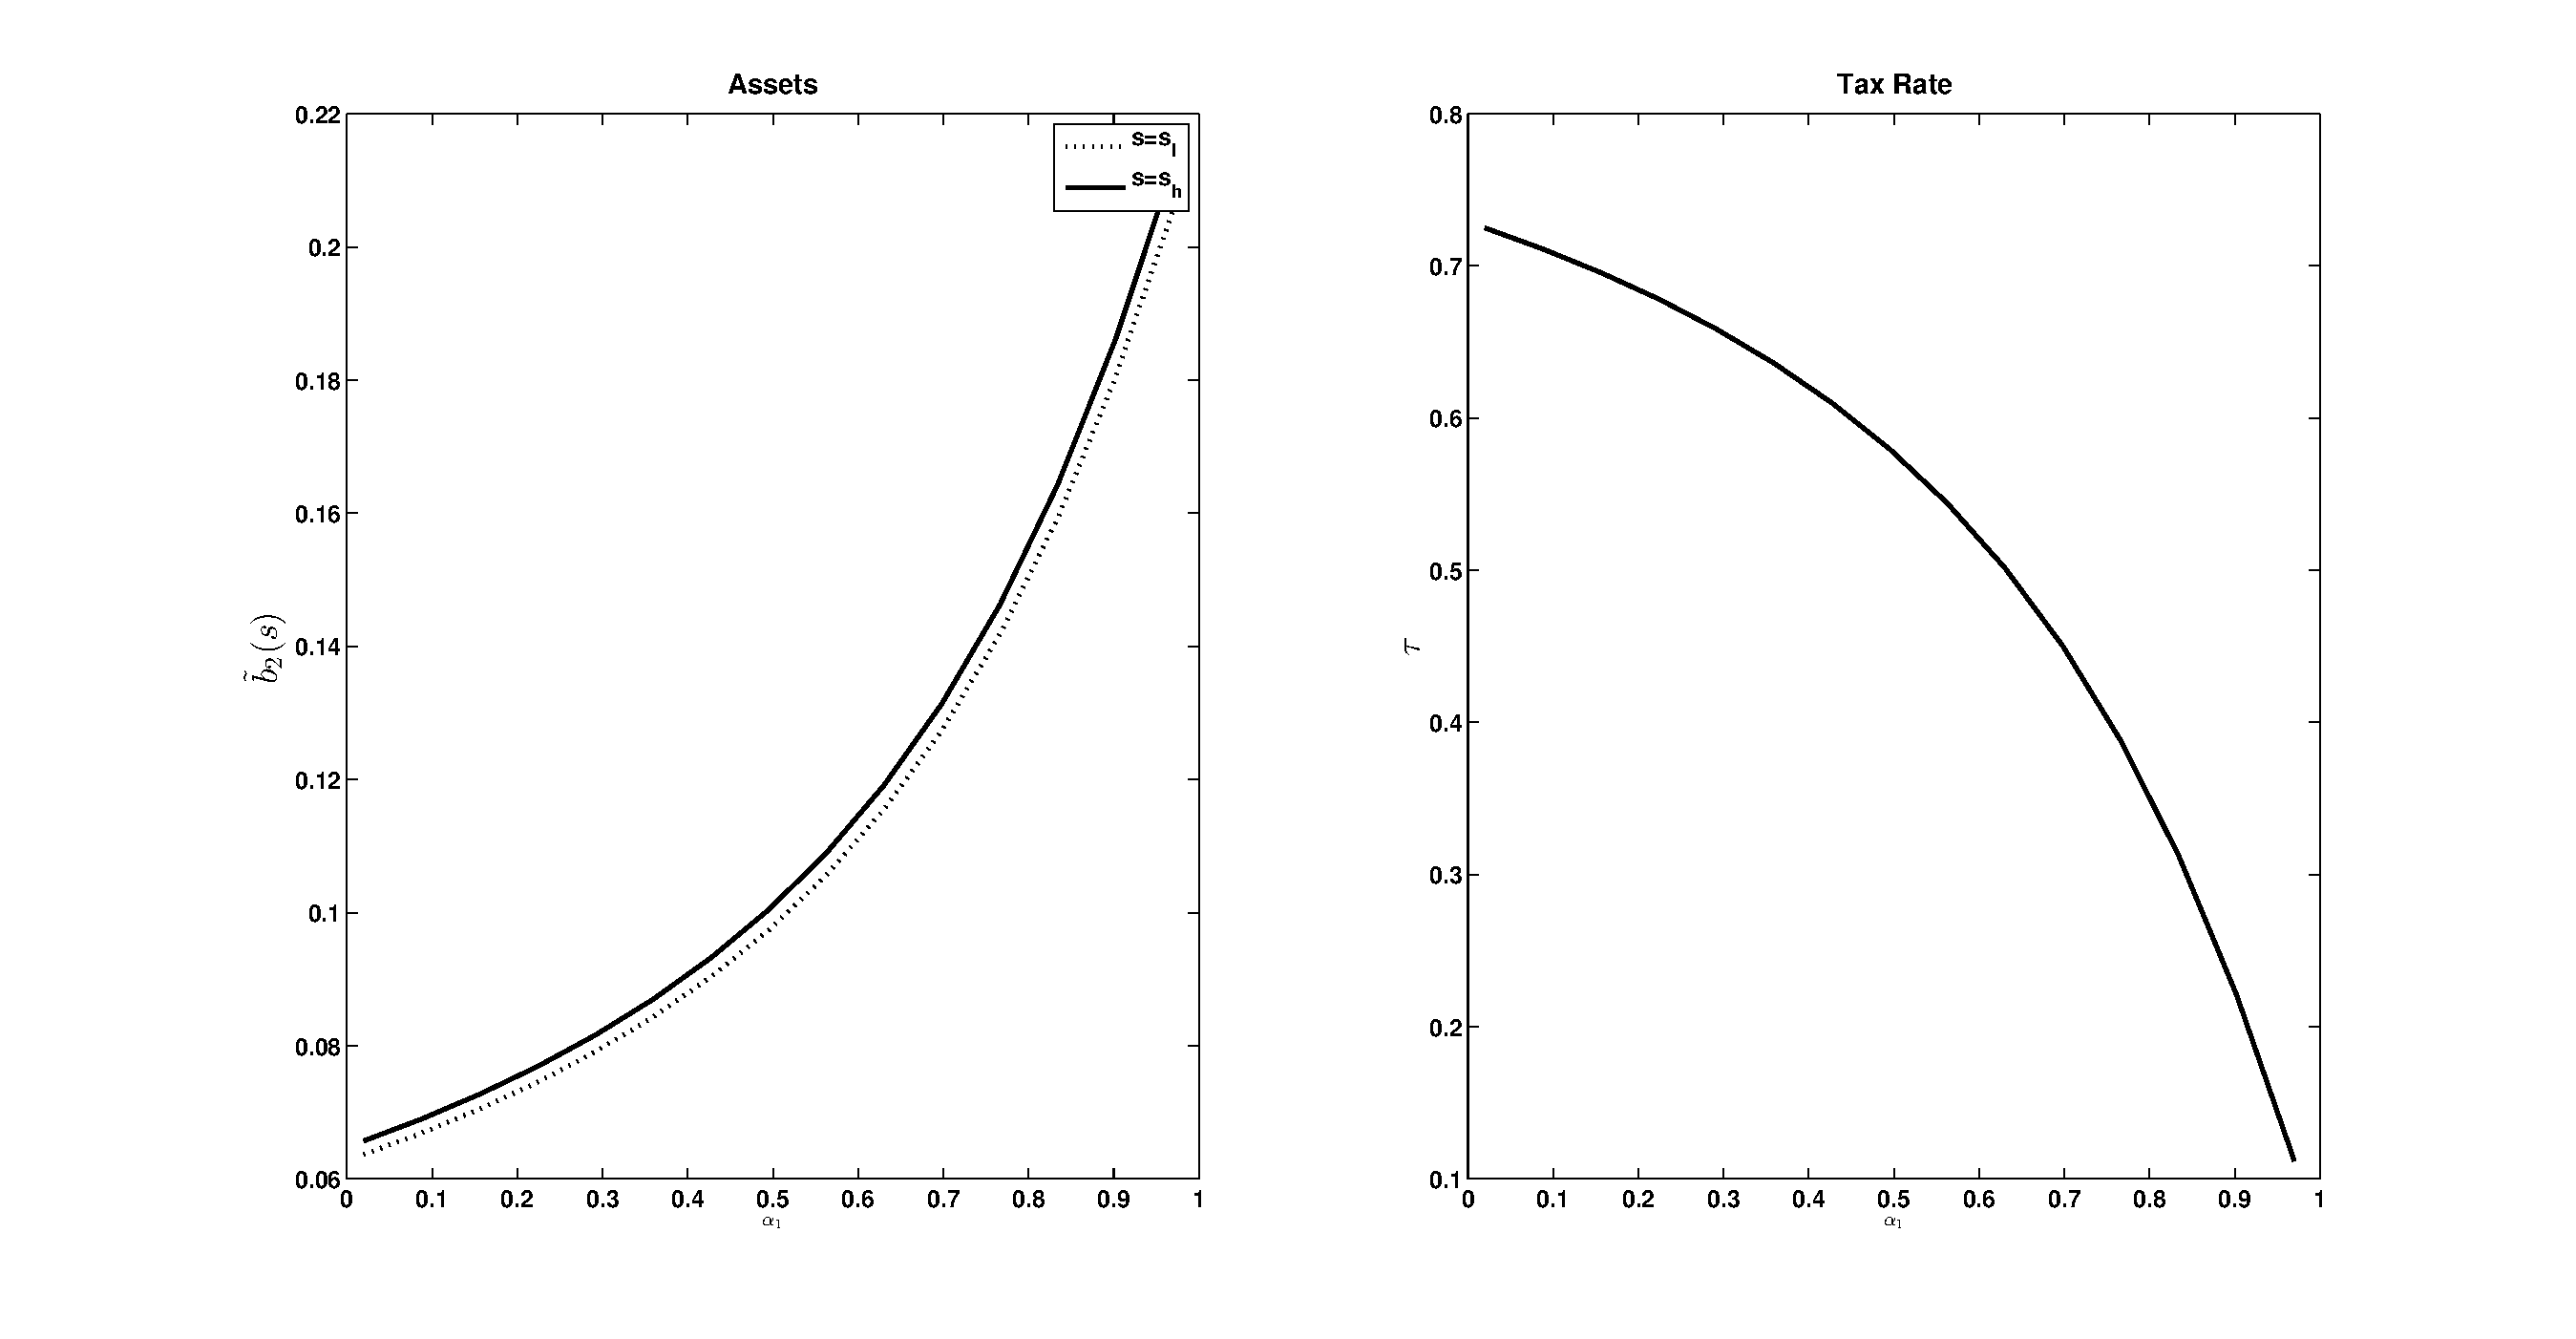
\includegraphics[width=\textwidth]{Draft25Graphs/SS_alpha1.eps}
%  \caption{Steady state govt. assets: $\tilde{b}_2(s)=\frac{\beta  x^{SS}}{U^2_c(s)}$ and taxes: $\tau^{SS}$ as a function of a (high skilled) agent 1's Pareto weight}
%  \label{fig: SS comparative}
%  \end{figure}
%
% \end{frame}

\begin{frame}
 \frametitle{Remarks on SS}
 \begin{itemize}
 \item Stability:
 \begin{enumerate}
  \item \textbf{Countercyclical interest rates:} Both forces push in the same direction $\rightarrow$ steady state is stable
  \item \textbf{Procyclical interest rates:} Both forces push in opposite direction $\rightarrow$ steady state is unstable
 \end{enumerate}
 \item For more than 2 agents, we have similar mechanics. In particular
  \begin{enumerate}
   \item Inequality distortions call for a negative correlation between productivities and (scaled) net assets
   \item Procyclical interest rates may flip the sign of the correlation between productivities and net assets to be positive.

   \begin{itemize}
   \item Low interest rate in recession prompts the government to hold debt
   \item By borrowing more from agents with higher productivities, the govt.\ can the reduce welfare costs of lowering transfers in adverse times
   \end{itemize}

  \end{enumerate}
\end{itemize}


\end{frame}

% \begin{frame}
% \frametitle{ case 1}
%
%
% Start with a spread in discount factors such that interest rates are equalized across i.e $R(s_l)=R(s_h)$. One can show that steady state $x>0$
%
% \begin{itemize}
%  \item The government can adjust two instruments in response  to an adverse  shock (i.e., a fall in $\theta_1$): it can either increase the  tax rate $\tau $ or it can decrease transfers $T.$ Both responses are distortionary
%  \item When agents' asset holdings are identical, a decrease in transfers  disproportionately
% affects a low-skilled agent, so his marginal utility falls by more than does the marginal utility of a high-skilled agent.
% \item  Consequently, a
% decrease in transfers increases inequality, giving rise to a cost  not present in  representative agent economies.
% \item  The government can reduce the costs of  inequality distortions by choosing tax rate policies that make the net asset positions of  the high-skilled agent
% decrease over time.
% \item this makes the two agents' after-tax and after-interest income  become closer, allowing decreases in transfers to have smaller effects on inequality in
% marginal utilities.
%  \end{itemize}
%
% \end{frame}

\begin{frame}
 \frametitle{Numerical Example}

 Use a  calibrated version of the economy to
 \begin{itemize}
  \item Approximate magnitudes of these forces and
  \item Study optimal policy responses at business cycle frequencies when an economy is possibly far away from a steady state
 \end{itemize}
 \end{frame}
 \begin{frame}
 \frametitle{Numerical Example: Calibration}
Take a 2-shock 2-type economy with preferences $U(c,l)=\psi \log(c)+(1-\psi)\log(1-l)$ and allow $\theta_i(s),\beta(s),g(s)$ to depend on $s$.

 \begin{itemize}

 \item Pick  baseline parameters to match some low frequency moments

 \item Calibrate outcome fluctuations to match three US recessions (i.e., 1991-92, 2001-02 and 2008-10):

 \begin{enumerate}
  \item Left tail of the cross-section distribution of labor income falls more than right tail
  \item Short term interest rate falls
  \item Booms last longer than recessions
 \end{enumerate}

 \end{itemize}

\end{frame}



\begin{frame}
 \frametitle{Calibration}

{\tiny
\begin{table}[htp]
{\tiny
\begin{tabular}{|l|l|l|c|}
\hline
Parameter & Value & Description &Target   \\ \hline
$\psi$ & 0.6994 &Frisch elasticity of labor supply & 0.5   \\
$\bar{\theta}_1 $ & 4& Log 90-10 wage ratio (Autor et al.) & 4   \\
$\bar{\theta}_2 $ & 1 &Normalize to 1 & 1  \\
$\beta$ & 0.98  &Average (annual) risk free interest rate & 2\%   \\
$\alpha_1$ & 0.69 & Marginal tax rate in the economy with no shocks & 20\% \\
$g$ & 12\%&Average pre-transfer expenditure-output ratio & 12\% \\
$\frac{\hat {\theta}_2}{\hat {\theta}_1}$ & 2.5 & Relative drop in wage income of 10th
percentile & 2.5\\
$\hat{\theta}_1$ & 1.2\% & Average output loss& 3\% \\
$\hat{\beta}(s)$ & 1.96\%& Difference in real interest rates between booms and recession& 1.96\% \\
$P(r|r)$ & 0.63&Duration of recessions & 2.33 years \\
$P(b|b)$ & 0.84 &Duration of booms &7 years \\ \hline
\end{tabular}
}
\caption{Benchmark calibration}
\label{tab:Parameters}
\end{table}
}
Initial conditions chosen to make  debt to GDP ratio be 60\% \footnote{We use the same normalization as before i.e, the low productive agent has zero assets}
 \end{frame}

\begin{frame}
 \frametitle{Results: Some variants }
 We study perturbations of the benchmark calibration
 \begin{enumerate}
\item \textbf{Acyclical interest rates}: smaller spread in discount factor shocks
\item \textbf{Countercyclical interest rates}: no discount factor shocks
\item \textbf{No inequality}: equal fall in all agents' productivities (TFP shock) and no discount factor shocks
%\item \textbf{Government expenditure shocks}: A fall in $g$ that produces a comparable fall in output
\end{enumerate}

 \end{frame}


\begin{frame}
 \frametitle{Results: Long run}

  \begin{figure}[htp]
 \centering
 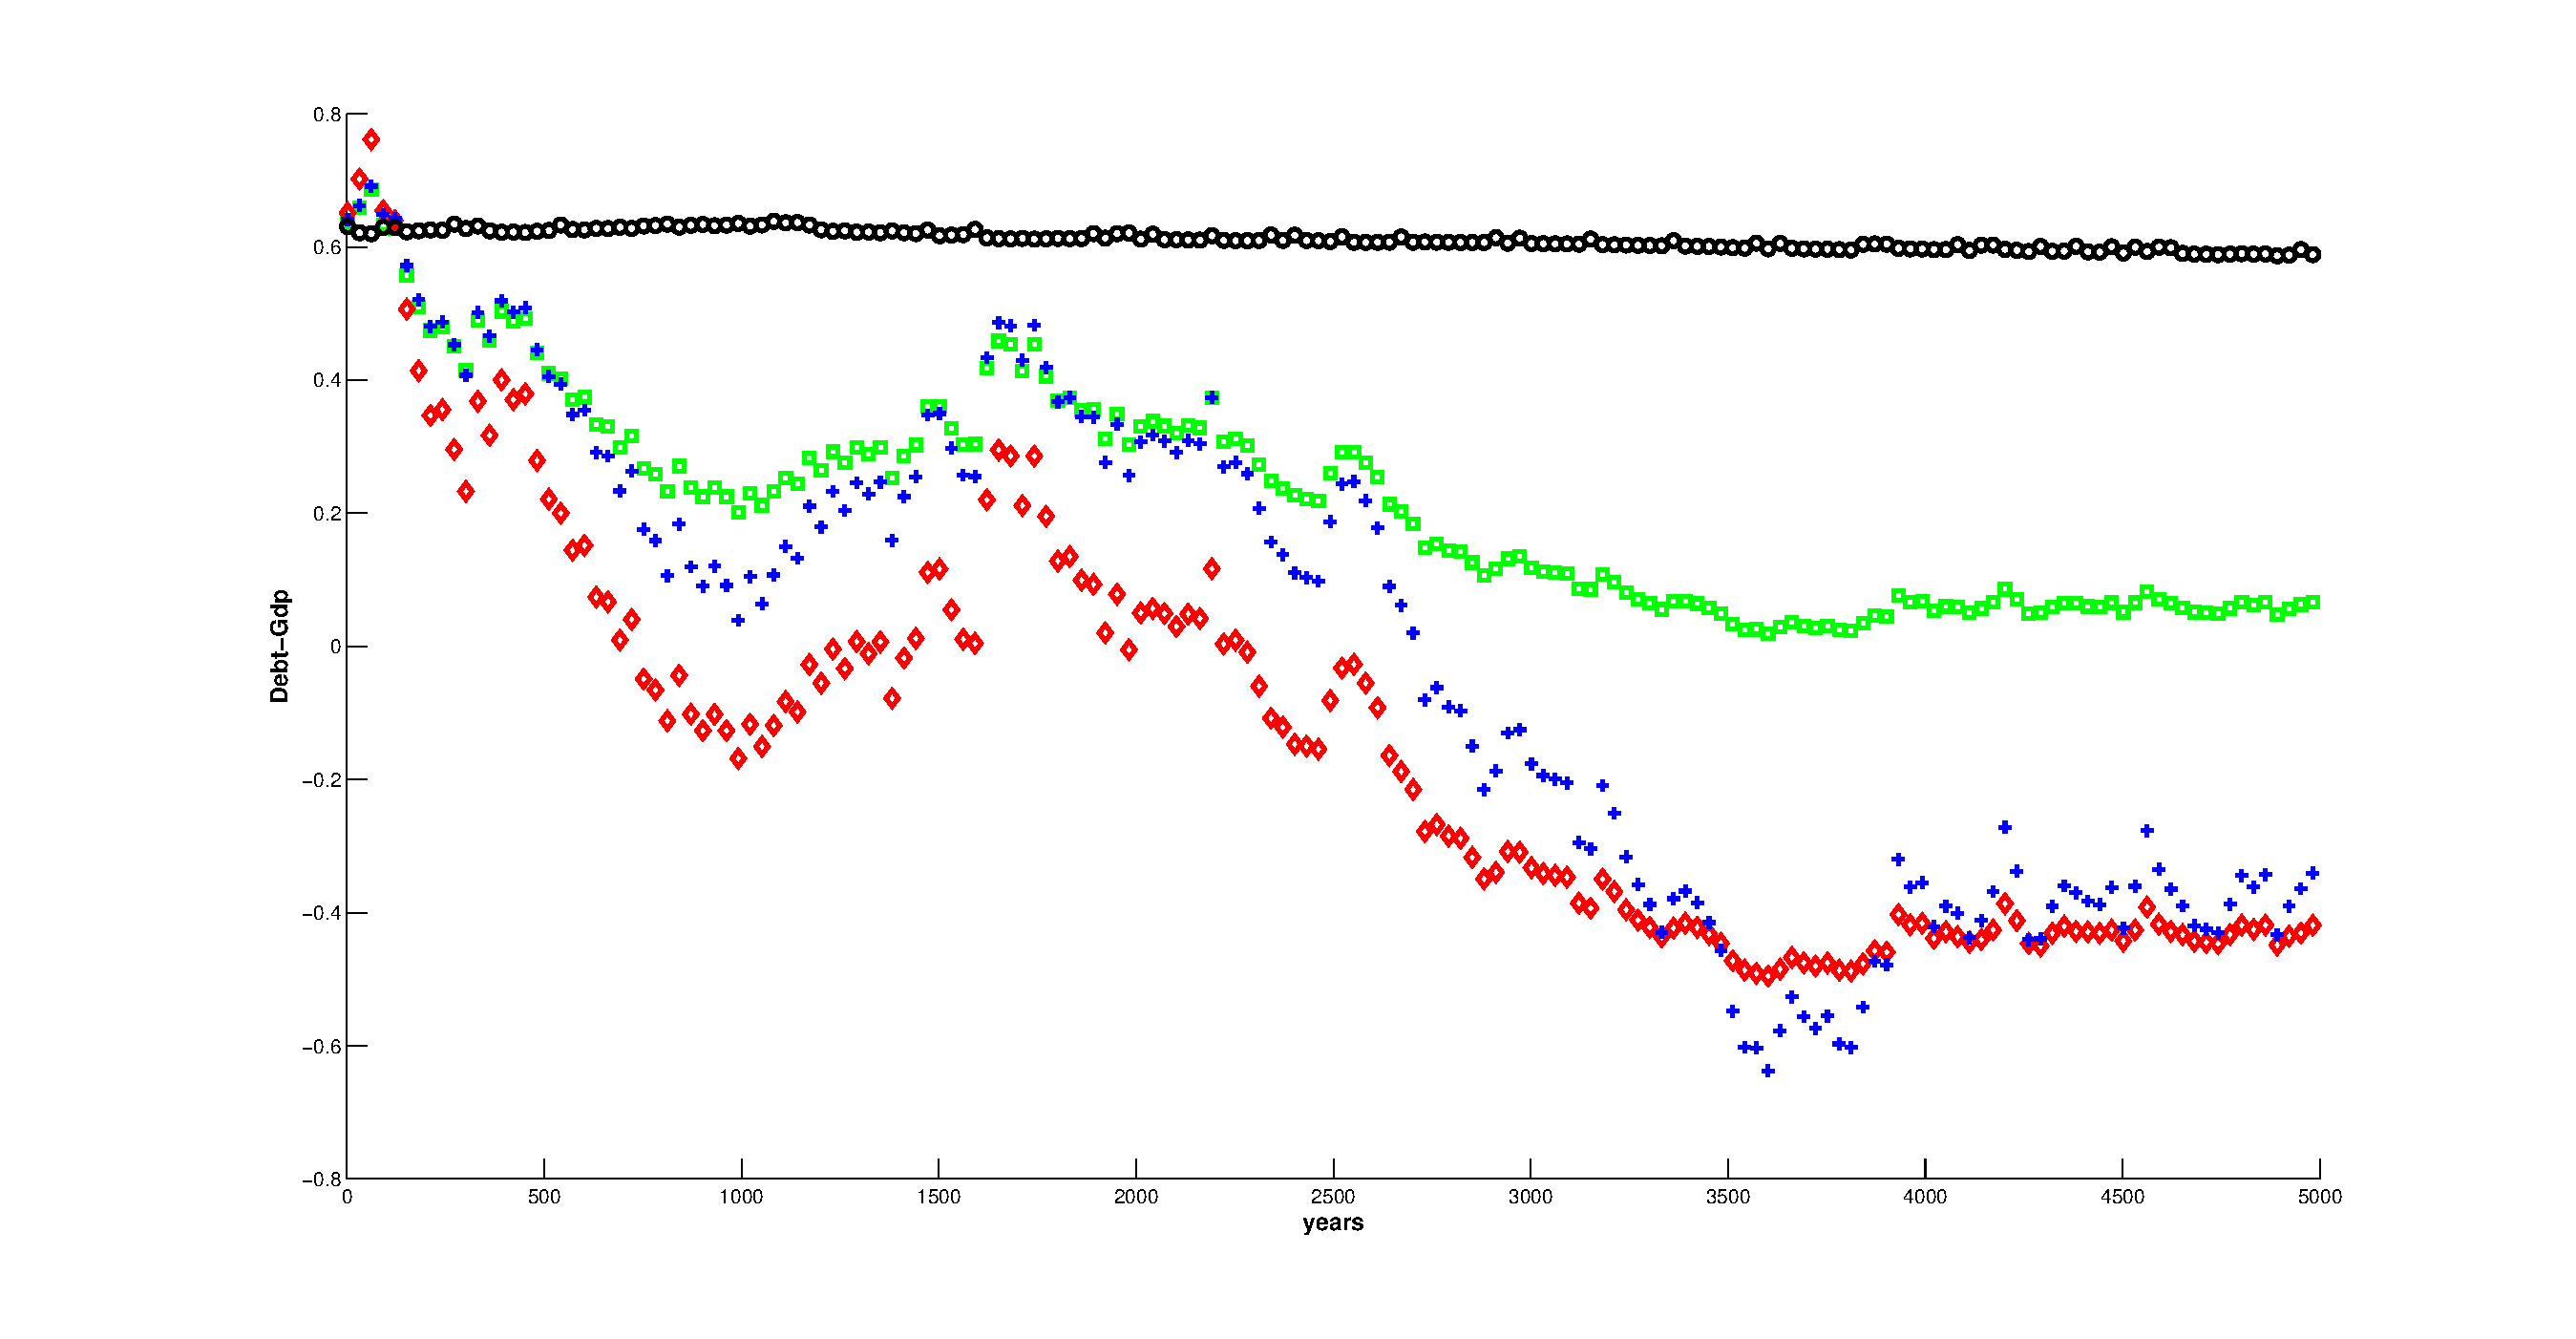
\includegraphics[width=\textwidth]{Draft25Graphs/LongSimulationsColor.eps}
 \caption{Govt. debt for several economies: benchmark (o), acyclical interest rates (\color{blue}+\color{black}), countercyclical interest rates (\color{red}$\diamond$\color{black}) and no inequality shocks \scriptsize (\color{green}$\square$\color{green}\normalsize) }
 %\caption{ Debt benchmark $\circle$, acyclical interest rates + , countercyclical interest rates $\diamond$ }% and no inequality shocks {\scriptsize $\square$ \normalsize}}
 \label{fig:LongSimulations}
 \end{figure}


 \end{frame}

 \begin{frame}[label=main]
  \frametitle{Observations}
  \begin{itemize}
   \item Long run tendency to converge to some ergodic set. But convergence is very slow
   \hyperlink{convergence}{\beamerbutton{more details on speed of convergence}}.
   \item With low discount factor shocks, outcomes approach positive govt. assets
   \item With high discount factor shocks that produce procyclical real interest rates, there is no tendency to reduce govt. debt even after 5000 years
  \end{itemize}

 \end{frame}

 \begin{frame}
  \frametitle{Short Run}
  To understand short run responses
  \begin{itemize}
   %\item   Set the exogenous state $s_0$ to put as at the onset of a recession
   \item Solve the time 0 problem with identical initial conditions across
different settings. This pins down the initial state vector  $x_0,\rho_0$  that appears in our time $0$ Bellman equation
\item Use  optimal policies to compute fluctuations of
different components in the government budget constraint as we move from booms to recessions
  \end{itemize}
 \end{frame}


 \begin{frame}
 \frametitle{Results: Short run}
 {\tiny
\begin{table}[tbp]
\begin{tabular}{|l|c|c|c|c|c|c|c|}
\hline
& \textbf{$\Delta g$} & \textbf{$\Delta B$} & \textbf{$\Delta T$} & \textbf{$%
\Delta [\tau\theta_1l_1]$} & \textbf{$\Delta [\tau\theta_2l_2]$} & \textbf{$%
\Delta Y$} & \textbf{$\Delta \tau$} \\ \hline
\textbf{Benchmark} & 0.0000 & -1.1561 & 0.6871 & -0.1593 & -0.3096 & -2.8536
& 0.3732 \\ \hline
\textbf{Acyclical Interest Rates} & 0.0000 & -1.1126 & 0.6591 & -0.1497 &
-0.3038 & -2.8613 & 0.3879 \\ \hline
\textbf{Countercyclical Interest Rates} & 0.0000 & -1.0794 & 0.6387 & -0.1415 &
-0.2992 & -2.8677 & 0.3997 \\ \hline
\textbf{No Inequality} & 0.0000 & -0.1380 &\color{red}{\textbf{ -0.5459}} & -0.5635 & -0.1204 &
-2.6294 & 0.0622 \\ \hline
%\textbf{Expenditure Shocks} & -7.5037 & 2.9137 & 2.8612 & -1.3759 & -0.3530 & -2.3443 &
%-1.1598 \\ \hline

\end{tabular}%

\caption{The table tells changes in different components of  government budget as the economy transits from ``boom'' to  ``recession''.  All numbers except $\protect\tau $ are normalized by undistorted GDP  and reported in percentages.
}

\label{tab:ShortRunPolicyResponses}
\end{table}
}
\begin{enumerate}
 \item For each variable
$z$ in the table we report  $\Delta z\equiv \left( z\left(
s_l|x_0,\rho_0,s_0\right) -z\left( s_h|x_0,\rho_0,s_0\right) \right) /\bar{Y}
$ where $\bar{Y}$ is average undistorted GDP in percentages
\item Predetermined variables like repayment on existing debt drop out
\begin{equation*}
\Delta [g]+\Delta[T]+ \Delta [B]=\Delta[\tau \theta_1 l_1]+ \Delta[\tau
\theta_2 l_2]
\end{equation*}%

\end{enumerate}

\small

 \end{frame}

\begin{frame}
 \frametitle{Concluding Remarks}
\begin{itemize}
\item Size of government debt alone is irrelevant $\Longrightarrow $
need to know   distribution of net assets
\item Optimal tax and transfer scheme balance
\begin{enumerate}
 \item welfare losses from fluctuating taxes
 \item welfare losses from fluctuating transfers
\end{enumerate}
%\item Since welfare costs depend on the how debt is distributed, the planner has incentives to move  net assets over time
\item With incomplete markets, interest rate fluctuations are a  key determinant of  long-run correlations between productivities and net assets
\item Ignoring heterogeneity produces misleading results about the size and direction of short run optimal policy responses
\end{itemize}

\end{frame}
\appendix
\section{More}

\begin{frame}[label=convergence]
\frametitle{Speed of convergence  (I) }
Suppose we are in the binary-IID world where steady states are deterministic.


\begin{itemize}
\item The optimal policy induces two \emph{risk adjusted} martingales
\begin{enumerate}
\item Multiplier on the implementability constraint : $\bm{\mu}_{t}$
\item The ratio of marginal utilities: $\bm{\rho}_{t}$
\end{enumerate}
 \item One can represent the optimal allocation recursively in terms of $\{\bm \mu(s^{t-1}),\bm \rho(s^{t-1})\}$ and $s_t$.
\item Why $(\bm{\mu},\bm{\rho})$ instead of $(\bm{x},\bm{\rho})$?
\item Linearize optimal policies for each $s_t$ around the constant steady state.
\item Study the eigenvalues of the conditional mean and variance dynamics (these are deterministic linear systems)
\end{itemize}

\end{frame}


\begin{frame}
\frametitle{Speed of convergence  (II) }
Let $\hat{\Psi}_{t}= \left[\bmat \bm{\mu}_{t} - \bm{\mu}^{SS}\\ \bm \rho_t - \bm \rho^{SS}\emat\right]$. Then
\begin{equation*}
 \hat{\Psi}_{t+1}=B(s_{t+1})\hat{\Psi}_t
\end{equation*}
This linearized system has coefficients that are functions of the shock $s$.
\small

\begin{proposition}\label{prop: localstability}
If the (real part) of eigenvalues of $\mathbb{E}B(s)$ are less than 1,  the system  converges to zero  in mean. Further for large $t$, the conditional variance of $\hat{\Psi}$, denoted by $\Sigma_{\Psi,t}$, follows a deterministic process governed by
\[\text{vec}(\Sigma_{\Psi,t})=\hat{B} \text{vec}(\Sigma_{\Psi,t-1}),\]	
where $\hat{B}$ is a square matrix of dimension $(2N-2)^2$. In addition,  if the (real parts) of eigenvalues of $\hat{B}$ are all less than 1, the system converges in probability.
\end{proposition}

\color{red}\emph{The eigenvalues (in particular the largest one) are instructive not only for whether the system is locally stable but also for how quickly the steady state is reached}

\end{frame}

\begin{frame}
\frametitle{Speed of convergence: Size of shocks and risk aversion}

  \begin{figure}[htp]
  \tiny
 \centering
 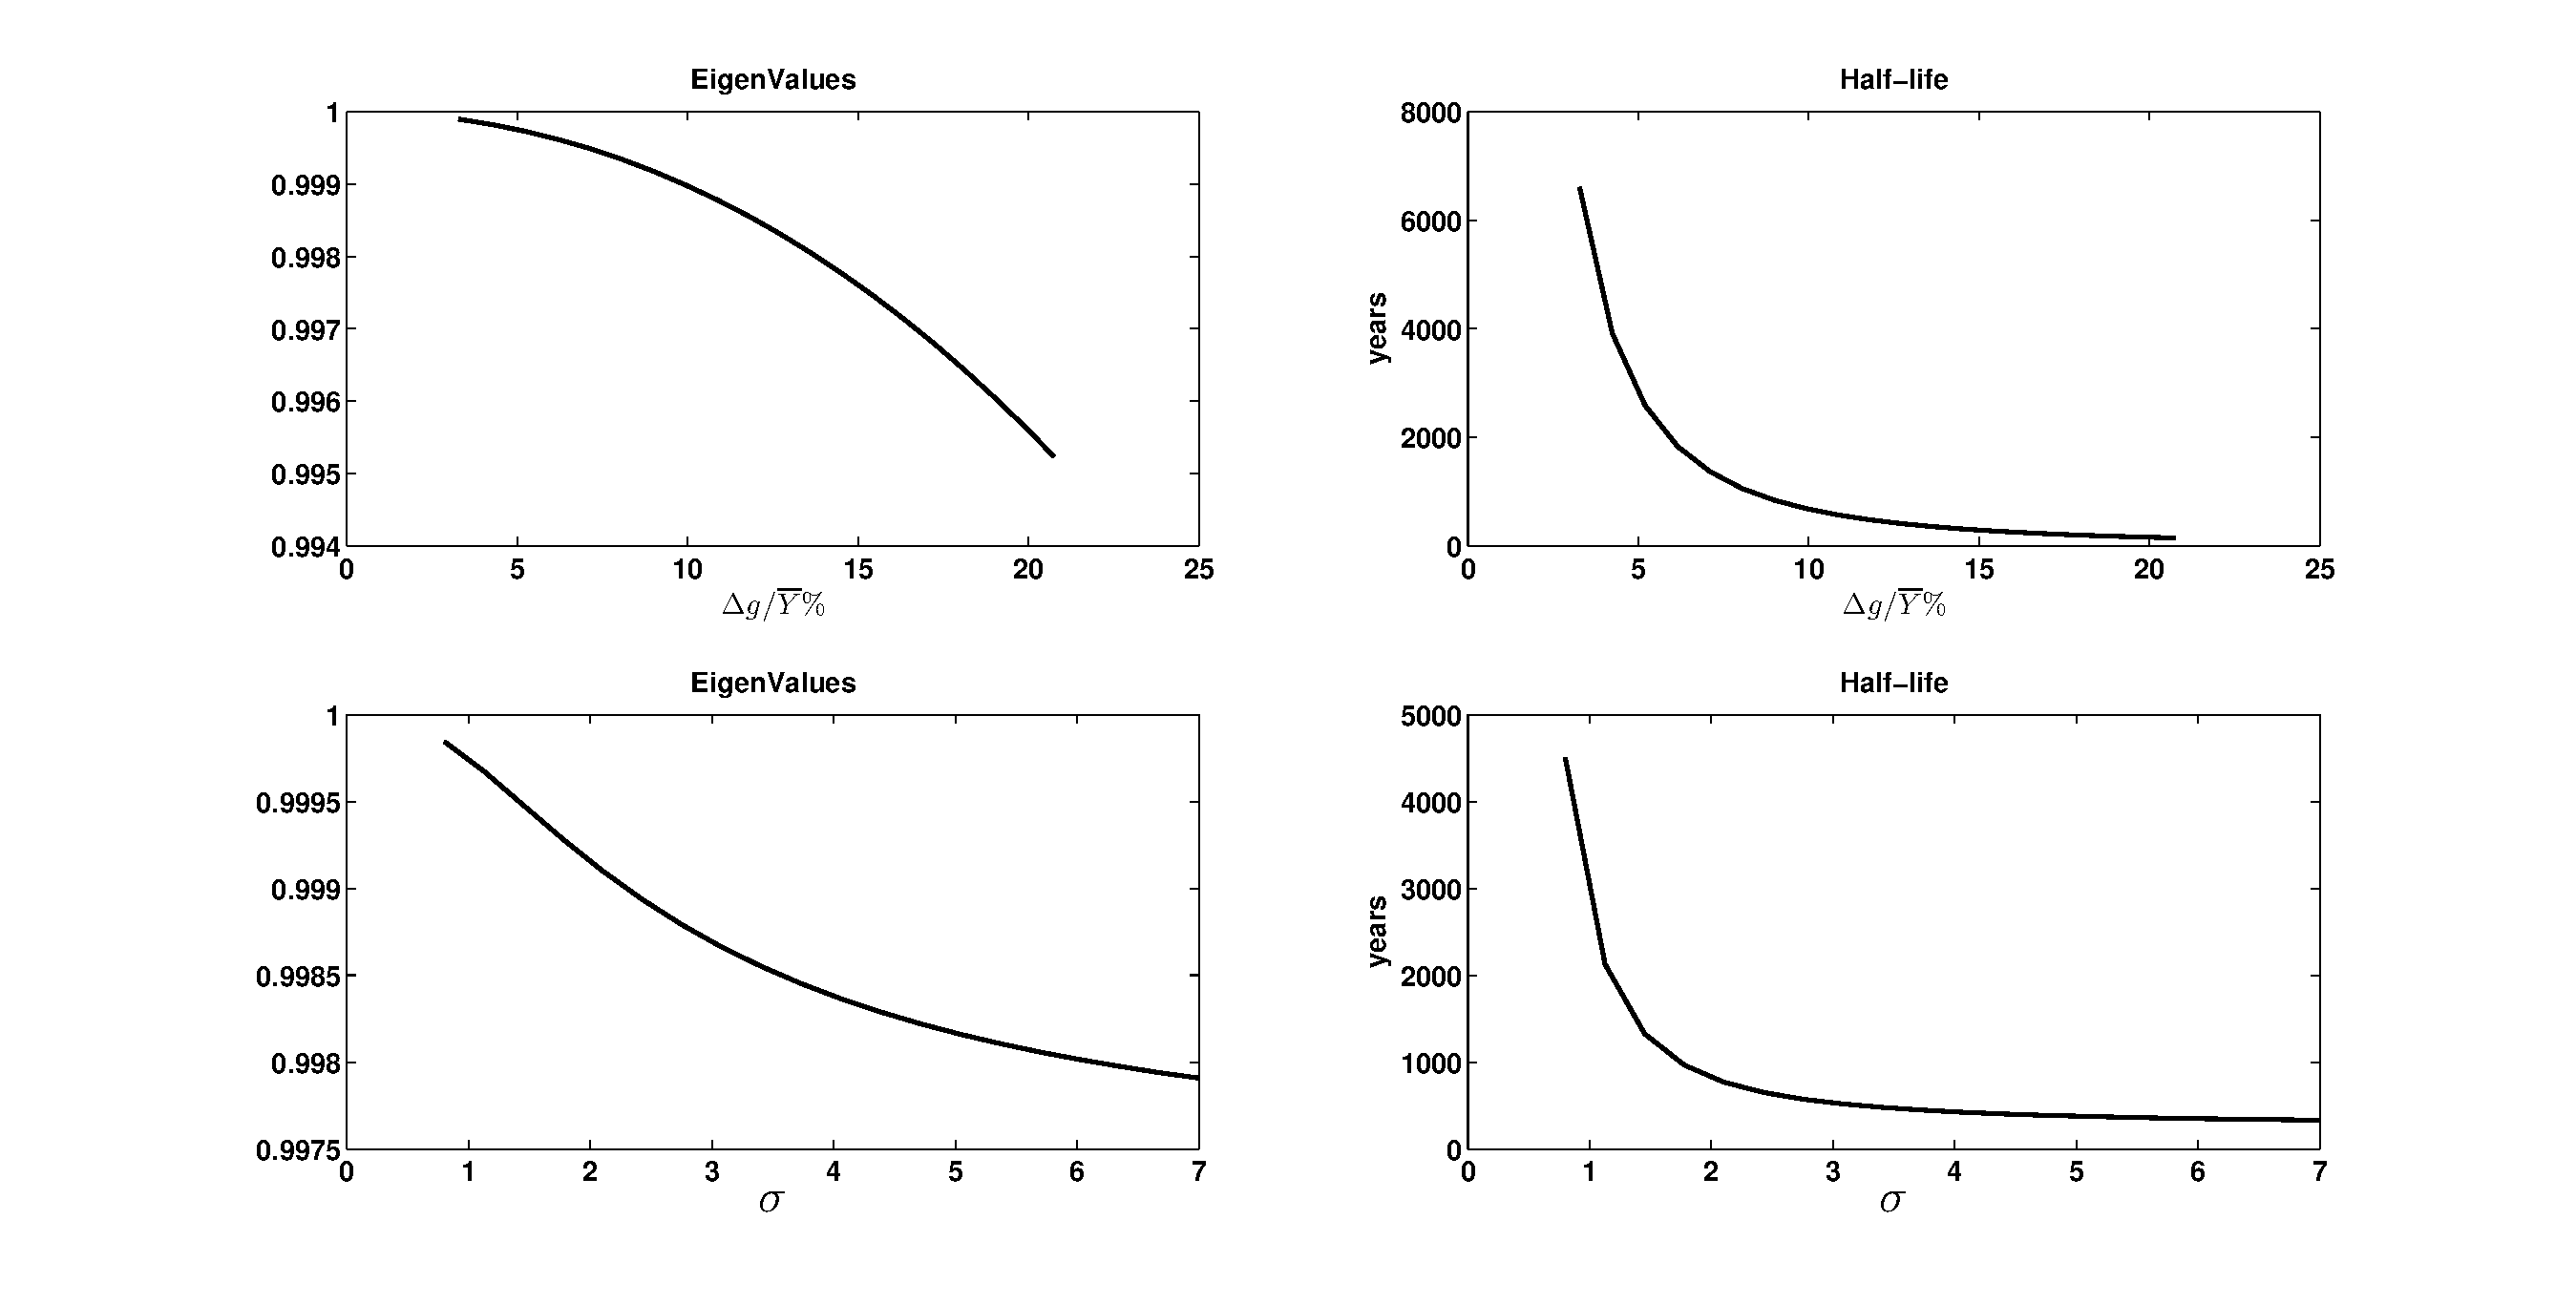
\includegraphics[width=\textwidth]{Draft25Graphs/eigenvalues.eps}
 \caption{\tiny{The top (bottom) panel plots the dominant eigenvalue of $\hat{B}$ and the associated half life as we increase
the spread between the expenditure levels (risk aversion).}}
 \label{fig: Eigenvalues}
 \end{figure}
 Back to \hyperlink{main}{\beamerbutton{main}}
 \end{frame}
 \end{document}

%
% \begin{itemize}
% \item Size of government debt alone is not informative $\Longrightarrow $
% need to know the net distribution of assets in the economy
%
% \item Ignoring heterogeneity produces misleading results about size and
% direction of the optimal policy response
%
% \item The better ability we have to tax assets, the less debt matters and
% can approximate complete markets closer
% \end{itemize}
%
% %TCIMACRO{\TeXButton{EndFrame}{\end{frame}}}%
% %BeginExpansion
% \end{frame}%
% %EndExpansion
%
% \end{document}
